\chapter{Cenni di complessità computazionale}\label{cap:compl}

\section{Problemi facili e difficili}

Prima di affrontare un problema di ottimizzazione occorre valutarne la \textbf{difficoltà}, che è legata agli algoritmi in grado di risolverlo:
\begin{itemize}[nosep]
\item \textbf{problema facile}: esiste un algoritmo \emph{polinomiale} che lo risolve;
\item \textbf{problema difficile}: non si conosce un algoritmo polinomiale che lo risolva.
\end{itemize}
La \textbf{complessità computazionale} studia la difficoltà dei problemi; servono due ingredienti: la \emph{dimensione dell'istanza} e la \emph{complessità degli algoritmi}.

\section{Istanza e dimensione dell'istanza}

\begin{defbox}[problema e istanza]
Un \textbf{problema} è una domanda generale, formulata su parametri simbolici. Un'\textbf{istanza} è un esempio specifico del problema, ottenuto fissando i valori numerici dei parametri.
\end{defbox}
Il problema dello zaino è ``dati $I,p,w,B$, risolvi $\max\{\sum p_ix_i:\sum w_ix_i\le B, x\in\{0,1\}^{|I|}\}$''; un'istanza è, per esempio, quella con gli 8 oggetti e $B=20$ di \S\ref{sec:zaino}.

\begin{defbox}[dimensione dell'istanza]
La \textbf{dimensione} di un'istanza è il numero di bit necessari a codificarla (in modo ``ragionevole'', cioè con i numeri in base 2 e non in unario).
\end{defbox}
Un intero $a$ richiede circa $\lceil\log_2(a+1)\rceil$ bit. Per lo zaino con $N=|I|$ oggetti:
\begin{center}
\begin{tabular}{@{}ll@{}}
\toprule
Dato & Bit \\ \midrule
numero di oggetti $N$ & $\lceil\log_2 N\rceil$\\
vettore dei profitti $p$ & $\sum_{i\in I}\lceil\log_2 p_i\rceil\le N\lceil\log_2 p_{\max}\rceil$\\
vettore dei pesi $w$ & $\sum_{i\in I}\lceil\log_2 w_i\rceil\le N\lceil\log_2 w_{\max}\rceil$\\
capacità $B$ & $\lceil\log_2 B\rceil$\\ \midrule
totale & $O\big(N(\log p_{\max}+\log w_{\max})+\log B\big)$\\
\bottomrule
\end{tabular}
\end{center}
Il punto chiave: la dimensione cresce \emph{linearmente} con il numero di oggetti ma solo \emph{logaritmicamente} con il valore dei numeri.

\section{Complessità degli algoritmi}

Un \textbf{algoritmo} è una sequenza finita di operazioni elementari che risolve un problema; per un problema di ottimizzazione, lo risolve se trova una soluzione ottima \emph{per ogni istanza}.

\begin{defbox}[complessità di un algoritmo]
La complessità di un algoritmo è la funzione che, per ogni dimensione $n$ dell'istanza, dà il numero di operazioni elementari (assegnamenti, confronti, operazioni aritmetiche) eseguite \textbf{nel caso peggiore} tra tutte le istanze di dimensione $n$.
\end{defbox}

\begin{esbox}[massima distanza tra $n$ punti]
Data la matrice delle distanze $\{d_{ij}\}$ tra $n$ punti, calcolare la distanza massima.
\begin{center}
\begin{tabular}{@{}ll@{}}
\texttt{dmax := 0} & 1 assegnamento\\
\texttt{per i = 1..n} & $n$ iterazioni\\
\quad\texttt{per j = 1..n} & $n$ iterazioni\\
\qquad\texttt{se d[i][j] > dmax} & 1 confronto\\
\qquad\quad\texttt{dmax := d[i][j]} & (al più) 1 assegnamento
\end{tabular}
\end{center}
Caso peggiore (le distanze arrivano in ordine crescente, quindi si aggiorna sempre): $1+2n^2$ operazioni, cioè $O(n^2)$. Sfruttando la simmetria ($j>i$) si fanno $n(n-1)/2$ iterazioni: ancora $O(n^2)$, cambia solo la costante. Nota che l'input ha $n^2$ numeri, quindi l'algoritmo è lineare nella dimensione dell'input.
\end{esbox}

\begin{defbox}[notazione $O$]
Date $f(n),g(n)$, si dice che $f(n)=O(g(n))$ se esistono $c>0$ e $n_0$ tali che $f(n)\le c\,g(n)$ per ogni $n>n_0$.
\end{defbox}
Si ignorano costanti moltiplicative e termini di ordine inferiore: $3n^2+10n+7=O(n^2)$.
\begin{itemize}[nosep]
\item \textbf{algoritmo polinomiale}: complessità $O(n^d)$ per qualche costante $d$;
\item \textbf{algoritmo esponenziale}: complessità del tipo $O(2^n)$ (o comunque non limitata da alcun polinomio).
\end{itemize}

\begin{center}
\begin{tabular}{@{}lrrrr@{}}
\toprule
$n$ & 10 & 20 & 50 & 100\\ \midrule
$n^2$ & 100 & 400 & 2\,500 & 10\,000\\
$n^3$ & 1\,000 & 8\,000 & 125\,000 & $10^6$\\
$2^n$ & 1\,024 & $\approx10^6$ & $\approx 10^{15}$ & $\approx10^{30}$\\
\bottomrule
\end{tabular}
\end{center}
A $10^9$ operazioni al secondo, $2^{100}$ operazioni richiedono circa $4\cdot10^{13}$ anni. Enumerare tutte le $2^N$ soluzioni dello zaino non è un'opzione.

\begin{extra}[algoritmi pseudo-polinomiali]
Lo zaino con dati interi si risolve con la programmazione dinamica: $F(k,b)$ = miglior profitto usando i primi $k$ oggetti con capacità $b$,
\[F(k,b)=\max\{F(k-1,b),\ F(k-1,b-w_k)+p_k\ (\text{se } w_k\le b)\},\qquad F(0,b)=0.\]
La tabella ha $N\cdot B$ celle: complessità $O(NB)$. Sembra polinomiale ma \textbf{non lo è}: $B$ è codificato con $\log_2B$ bit, quindi $O(NB)=O(N\,2^{\log_2B})$ è esponenziale nella dimensione dell'input. Un algoritmo polinomiale nel \emph{valore} dei numeri (non nella loro lunghezza) si dice \emph{pseudo-polinomiale}. Utile in pratica se $B$ è piccolo; non contraddice la NP-completezza dello zaino.
\end{extra}

\section{Problemi di riconoscimento}

La teoria si sviluppa per problemi con risposta SÌ/NO.
\begin{defbox}[versione di riconoscimento]
La \textbf{versione di riconoscimento} (o decisionale) di un problema di ottimizzazione $\max\{cx: Ax\le b,\ x\ge0,\ x\in\Z^n\}$, data una soglia $k$, chiede:
\[ \exists\,x:\ Ax\le b,\ x\ge 0,\ x\in\Z^n,\ cx\ge k\ ? \]
(per un minimo: $cx\le k$).
\end{defbox}
\textbf{Zaino (riconoscimento):} dati oggetti con profitti $p_i$, pesi $w_i$, capacità $B$ e soglia $k$, esiste un sottoinsieme di oggetti di peso complessivo $\le B$ e profitto complessivo $\ge k$?

\begin{oss}[perché basta studiare il riconoscimento]
Se so risolvere l'ottimizzazione, so rispondere al riconoscimento (confronto il valore ottimo con $k$). Viceversa, con dati interi il valore ottimo sta in un intervallo $[L,U]$ con $\log(U-L)$ polinomiale nella dimensione: con una \emph{ricerca binaria} su $k$ bastano polinomialmente molte chiamate al riconoscimento. Quindi le due versioni sono ``ugualmente difficili'' a meno di un fattore polinomiale.
\end{oss}

\section{Le classi \texorpdfstring{$\Pc$}{P} e \texorpdfstring{$\NP$}{NP}}

\begin{defbox}[classe $\Pc$]
Un problema appartiene a $\Pc$ se esiste un algoritmo che, per ogni istanza del problema di riconoscimento, decide in tempo polinomiale se la risposta è SÌ o NO. (Il corrispondente problema di ottimizzazione si risolve all'ottimo in tempo polinomiale.)
\end{defbox}

\begin{defbox}[classe $\NP$]
Un problema appartiene a $\NP$ se, per ogni istanza con risposta SÌ, esiste un \textbf{certificato} $\gamma(I)$ (tipicamente una soluzione) di dimensione polinomiale e un algoritmo $A$ che verifica \textbf{in tempo polinomiale} che $\gamma(I)$ attesta la risposta SÌ.
\end{defbox}
In parole: \emph{trovare} la soluzione può essere difficile, ma \emph{controllarla} è facile.

\begin{itemize}[nosep]
\item $\NP$ significa \textbf{Non-deterministico Polinomiale} (una macchina che ``indovina'' il certificato e poi lo verifica), \textbf{non} ``non polinomiale''!
\item $\Pc\subseteq\NP$: se il problema è in $\Pc$, il verificatore può ignorare il certificato e risolvere l'istanza da zero in tempo polinomiale.
\item Se $\Pc\subsetneq\NP$ oppure $\Pc=\NP$ è uno dei grandi problemi aperti della matematica (uno dei Millennium Prize Problems). Si congettura $\Pc\ne\NP$.
\end{itemize}

\begin{esbox}[lo zaino è in $\NP$]
Certificato: il sottoinsieme $S$ di oggetti (un vettore $x\in\{0,1\}^N$, dimensione $N$). Verifica: calcolo $\sum_{i\in S}w_i$ e lo confronto con $B$; calcolo $\sum_{i\in S}p_i$ e lo confronto con $k$. Sono $O(N)$ somme e 2 confronti: tempo polinomiale.
\end{esbox}
Notare l'asimmetria: per certificare una risposta NO (``nessun sottoinsieme raggiunge $k$'') non si conosce un certificato breve.

\section{Riduzioni e \texorpdfstring{$\NP$}{NP}-completezza}

\begin{defbox}[riduzione polinomiale]
Dati due problemi $P_1$ e $P_2$, $P_1$ \textbf{si riduce in tempo polinomiale} a $P_2$ ($P_1\red P_2$) se per ogni istanza $I_1$ di $P_1$ si può costruire in tempo polinomiale un'istanza $I_2$ di $P_2$ tale che dalla soluzione di $I_2$ si ricava in tempo polinomiale la soluzione di $I_1$.
\end{defbox}

\begin{center}
\begin{tikzpicture}[>=Stealth, box/.style={draw,rounded corners,minimum height=0.8cm,font=\small,fill=gray!8}]
\node[box] (i1) {$I_1$ (istanza di $P_1$)};
\node[box,right=1.2cm of i1] (i2) {$I_2$};
\node[box,right=1.2cm of i2] (a2) {algoritmo $A_2$};
\node[box,right=1.2cm of a2] (s1) {soluzione di $I_1$};
\draw[->] (i1)--node[above,font=\scriptsize]{poly} (i2);
\draw[->] (i2)--(a2);
\draw[->] (a2)--node[above,font=\scriptsize]{poly} (s1);
\draw[dashed,rounded corners] ($(i1.north west)+(-0.2,0.5)$) rectangle ($(s1.south east)+(0.2,-0.3)$);
\node[font=\scriptsize,fill=white] at ($(i2)!0.5!(a2)+(0,0.8)$) {algoritmo $A_1$ per $P_1$};
\end{tikzpicture}
\end{center}

Conseguenze:
\begin{itemize}[nosep]
\item se esiste un algoritmo $A_2$ per $P_2$, ottengo un algoritmo $A_1$ per $P_1$ che usa $A_2$; se $A_2$ è polinomiale, lo è anche $A_1$;
\item se $P_1\red P_2$, allora \textbf{$P_2$ è almeno tanto difficile quanto $P_1$};
\item se $P_1\red P_2$ e $P_2\in\Pc$, allora $P_1\in\Pc$;
\item (contronominale) se $P_1\red P_2$ e $P_1$ è difficile, allora anche $P_2$ è difficile.
\end{itemize}

\begin{esame}
\textbf{Il verso della riduzione} è l'errore più comune. Per dimostrare che un problema \emph{nuovo} $P$ è difficile si riduce un problema \emph{noto} difficile \emph{a} $P$: $P_{\text{noto}}\red P$ (``se sapessi risolvere $P$ saprei risolvere anche il problema noto''). Ridurre $P$ a un problema difficile ($P\red P_{\text{noto}}$) non dice nulla sulla difficoltà di $P$: tutto si riduce a un problema difficile.
\end{esame}

\begin{defbox}[$\NP$-completo]
Un problema $P$ è \textbf{$\NP$-completo} se
\begin{enumerate}[label=\roman*),nosep]
\item $P\in\NP$;
\item $P_1\red P$ per ogni $P_1\in\NP$.
\end{enumerate}
Cioè $P$ è almeno tanto difficile quanto ogni altro problema in $\NP$. Se vale solo ii), $P$ si dice $\NP$-\emph{difficile} (\emph{NP-hard}); si usa questo termine per le versioni di ottimizzazione, che non sono problemi SÌ/NO.
\end{defbox}
Per i problemi $\NP$-completi non si conosce un algoritmo polinomiale che garantisca l'ottimo per ogni istanza. Se se ne trovasse uno per \emph{un} solo problema $\NP$-completo, allora $\Pc=\NP$.

\textbf{Come si dimostra che $P$ è $\NP$-completo} (senza ridurre ogni problema di $\NP$ uno per uno):
\begin{enumerate}[nosep]
\item si dimostra che $P\in\NP$ (esibendo certificato e verifica polinomiale);
\item si dimostra che $P_1\red P$ per \emph{un} problema $P_1$ già noto come $\NP$-completo.
\end{enumerate}
\begin{prop}
La riducibilità è transitiva: $P'\red P_1$ e $P_1\red P$ implicano $P'\red P$. Quindi i passi 1--2 bastano.
\end{prop}
\begin{dimo}
Transitività: si compongono le due trasformazioni; la composizione di funzioni polinomiali è polinomiale (un polinomio di un polinomio è un polinomio, e l'output di una trasformazione polinomiale ha dimensione polinomiale). Poiché $P_1$ è $\NP$-completo, $P'\red P_1$ per ogni $P'\in\NP$; per transitività $P'\red P$ per ogni $P'\in\NP$; con $P\in\NP$ si conclude. \hfill$\square$
\end{dimo}

\begin{center}
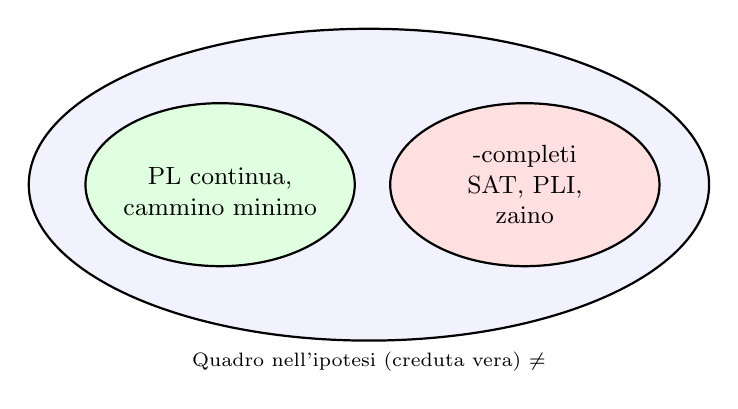
\begin{tikzpicture}[scale=0.9]
\draw[thick,fill=blue!5] (0,0) ellipse (4.8 and 2.2);
\node at (0,1.7) {$\NP$};
\draw[thick,fill=green!12] (-2.1,0) ellipse (1.9 and 1.15);
\node[align=center,font=\small] at (-2.1,0) {$\Pc$\\ PL continua,\\ cammino minimo};
\draw[thick,fill=red!12] (2.2,0) ellipse (1.9 and 1.15);
\node[align=center,font=\small] at (2.2,0) {$\NP$-completi\\ SAT, PLI,\\ zaino};
\node[font=\scriptsize,align=center] at (0,-2.5) {Quadro nell'ipotesi (creduta vera) $\Pc\neq\NP$};
\end{tikzpicture}
\end{center}

\section{Il problema della soddisfacibilità (SAT)}

Il primo problema dimostrato $\NP$-completo (Cook, 1971, con una dimostrazione ``diretta'' che simula una macchina di Turing) è la \textbf{soddisfacibilità}.
\begin{defbox}[SAT]
Date $n$ variabili booleane $y_1,\dots,y_n$ e $m$ espressioni booleane (\emph{clausole}) $C_1,\dots,C_m$, ciascuna disgiunzione ($\lor$) di letterali (variabili o loro negazioni $\bar y_i$), ad esempio $C_1=y_1\lor y_2\lor\bar y_3$, esiste un assegnamento di valori di verità alle variabili che renda \emph{tutte} le clausole vere?
\end{defbox}
Esempio: $(y_1\lor y_2\lor\bar y_3)\land(\bar y_1\lor y_3)\land(\bar y_2\lor\bar y_3)$ è soddisfatta da $y_1=1,y_2=0,y_3=1$.

\section{La Programmazione Lineare Intera è \texorpdfstring{$\NP$}{NP}-completa}

\begin{prop}
La versione di riconoscimento di un generico problema di PLI
\[ \exists x:\ Ax\le b,\ x\ge0,\ x\in\Z^n,\ cx\le k\ ? \]
è $\NP$-completa.
\end{prop}

\textbf{1) PLI $\in\NP$.} Data una soluzione $x$ come certificato, bisogna: controllare tutti i vincoli ($m$ prodotti scalari, $O(mn)$ operazioni) e l'interezza; calcolare $cx$ e confrontarlo con $k$. Tutto in tempo polinomiale. (Sottigliezza tecnica, non richiesta: si dimostra che se esiste una soluzione intera ammissibile ne esiste una con componenti di dimensione polinomiale, quindi il certificato è ``corto''.)

\textbf{2) SAT $\red$ PLI.} Data un'istanza di SAT costruiamo un'istanza di PLI:
\begin{center}
\begin{tabular}{@{}ll@{}}
\toprule
Istanza SAT & Istanza PLI\\ \midrule
variabile booleana $y_i$ & variabile $x_i\in\{0,1\}$ (cioè $0\le x_i\le1$, $x_i\in\Z$)\\
letterale $y_i$ & $x_i$\\
letterale $\bar y_i$ & $1-x_i$\\
clausola $y_1\lor y_2\lor\bar y_3$ vera & $x_1+x_2+(1-x_3)\ge1$\\
\bottomrule
\end{tabular}
\end{center}
In generale, per la clausola $C_j$ con letterali positivi $P_j$ e negati $N_j$:
\[ \sum_{i\in P_j}x_i+\sum_{i\in N_j}(1-x_i)\ge 1\qquad \forall j=1,\dots,m, \]
cioè ``almeno un letterale della clausola è vero''. Obiettivo irrilevante: $c=0$, $k=0$ (la domanda diventa ``esiste una soluzione ammissibile?'').

\emph{Correttezza}: un assegnamento di verità soddisfa tutte le clausole se e solo se il corrispondente vettore 0/1 soddisfa tutti i vincoli. \emph{Tempo}: una variabile per variabile booleana e un vincolo per clausola: la costruzione è lineare nella dimensione dell'istanza SAT; la risposta si trasferisce identica.

\begin{esbox}[istanza costruita]
$(y_1\lor y_2\lor\bar y_3)\land(\bar y_1\lor y_3)\land(\bar y_2\lor\bar y_3)$ diventa
\[ x_1+x_2-x_3\ge0,\qquad -x_1+x_3\ge0,\qquad -x_2-x_3\ge-1,\qquad x\in\{0,1\}^3. \]
$x=(1,0,1)$ è ammissibile, coerentemente con l'assegnamento trovato prima.
\end{esbox}

\begin{esbox}[un'altra riduzione: Subset Sum $\red$ Zaino]
\textsc{Subset Sum} ($\NP$-completo): dati interi $a_1,\dots,a_N$ e $T$, esiste un sottoinsieme con somma esattamente $T$? Costruisco l'istanza di zaino con $p_i=w_i=a_i$, $B=k=T$. Un sottoinsieme ha peso $\le T$ e profitto $\ge T$ se e solo se ha somma esattamente $T$. Costruzione lineare, quindi lo zaino (riconoscimento) è $\NP$-completo.
\end{esbox}

\section{Conseguenze pratiche}

\begin{itemize}
\item \textbf{PL con variabili continue è in $\Pc$} (metodo dell'ellissoide, Khachiyan 1979; metodi a punto interno, Karmarkar 1984). Il simplesso, curiosamente, ha complessità esponenziale nel caso peggiore (esempi di Klee--Minty) ma è velocissimo in pratica.
\item \textbf{PLI e PLMI sono $\NP$-difficili}. Aggiungere il vincolo di interezza cambia radicalmente la difficoltà: è il motivo per cui nei modelli si usano variabili intere solo quando servono.
\item $\NP$-completo non vuol dire ``irrisolvibile'': molte istanze reali si risolvono bene con metodi esatti (branch-and-bound, piani di taglio) che sfruttano i rilassamenti, oppure si usano euristiche (soluzioni buone senza garanzia di ottimalità).
\item Un problema specifico può essere facile anche se la sua formulazione naturale è una PLI (es.\ cammino minimo, assegnamento, flussi su grafo): la PLI è $\NP$-completa come \emph{classe}, non ogni sua istanza o sottoclasse. Si vedrà nella parte sui grafi.
\end{itemize}

\begin{esame}
Domande teoriche tipiche: definire istanza, dimensione, complessità di un algoritmo (caso peggiore); definire $\Pc$, $\NP$, riduzione, $\NP$-completo; spiegare perché $\Pc\subseteq\NP$; mostrare che un problema è in $\NP$ (certificato + verifica); scrivere la riduzione SAT $\red$ PLI; spiegare il verso di una riduzione.
\end{esame}
